\documentclass{article}
\usepackage{amsmath}
\usepackage{amsfonts}
\usepackage{graphicx}
\usepackage{tikz}

\begin{document}

\section*{Ejercicio 1, S-T eficientes, Daniel Bustos}

Dado un digrafo \( D \) con pesos \( c : E(D) \to \mathbb{N} \) y dos vértices \( s \) y \( t \), decimos que una arista \( v \to w \) es \textit{st-eficiente} cuando \( v \to w \) pertenece a algún camino mínimo de \( s \) a \( t \). Sea \( d(\cdot, \cdot) \) la función que indica el peso de un camino mínimo entre dos vértices.

\subsection*{a. Demostrar que \( v \to w \) es st-eficiente \(\leftrightarrow\) \( d(s, v) + c(v \to w) + d(w, t) = d(s, t) \)}

\textbf{Ida:}

Si \( v \to w \) es st-eficiente, entonces pertenece a un camino mínimo. Podemos tomar ese camino y reescribir su costo total como:
\[ d(s, v) + c(v \to w) + d(w, t) = d(s, t) \]

\textbf{Vuelta:}

Si \( d(s, v) + c(v \to w) + d(w, t) = d(s, t) \), luego por definición pertenece a un camino mínimo, ya que la distancia es la misma. Entonces, \( v \to w \) es st-eficiente.

\subsection*{b. Algoritmo para encontrar el camino mínimo que no use aristas st-eficientes}

Usando el inciso anterior, proponga un algoritmo eficiente que encuentre el mínimo de los caminos entre \( s \) y \( t \) que no use aristas st-eficientes. Si dicho camino no existe, el algoritmo retorna \(\perp\).

\textbf{Algoritmo:}
\begin{enumerate}
    \item Ejecutamos el algoritmo de Dijkstra con raíz en \( s \) . Luego sobre  de nuevo con raíz en \( t \) sobre el grafo transpuesto.
    \item Usando la fórmula anterior, iteramos por todas las aristas y verificamos si son o no st-eficientes dado que los algoritmos previos nos dicen las distancias d(s,v) y d(t,v) para un vertice v cualquiera. Las que no lo son, las incluimos en otro grafo con la misma cantidad de vértices.
    \item Ejecutamos Dijkstra sobre este otro grafo, con raíz en \( s \), y retornamos el camino mínimo.
\end{enumerate}

Observemos que este camino podría no existir, ya que tal vez los únicos caminos en el grafo original son mínimos, dejándonos sin aristas no st-eficientes.

Complejidad : $3*\Theta (m + n*log(n)) \ + 2* (\ n + \ m) = \Theta (m + n*log(n)) $

\newpage
\subsection*{Ejemplo con gráficos}

A continuación, se presentan gráficos para ejemplificar la idea:

\begin{figure}[h]
    \centering
    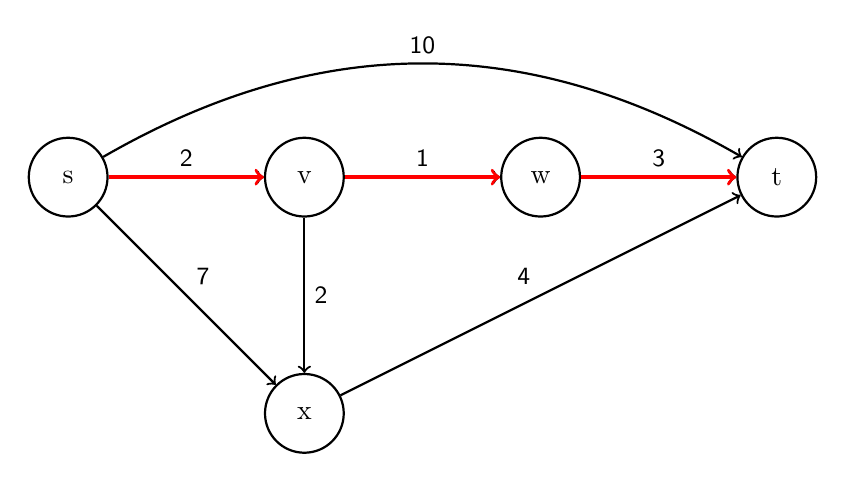
\begin{tikzpicture}[->, auto, node distance=3cm, thick, main node/.style={circle, draw, minimum size=1cm}]
        \node[main node] (s) {s};
        \node[main node] (v) [right of=s] {v};
        \node[main node] (w) [right of=v] {w};
        \node[main node] (t) [right of=w] {t};
        \node[main node] (x) [below of=v] {x};

        \path[every node/.style={font=\sffamily\small}]
 	    (s) edge node {7} (x)        
        (s) edge node {2} (v)
        (v) edge node {1} (w)
        (w) edge node {3} (t)
        (v) edge node {2} (x)
        (x) edge node {4} (t)
        (s) edge [bend left] node {10} (t);

        \draw[red, very thick] (s) -- (v);
        \draw[red, very thick] (v) -- (w);
        \draw[red, very thick] (w) -- (t);

    \end{tikzpicture}
    \caption{Camino mínimo original (aristas rojas)}
    \label{fig:original}
\end{figure}

\begin{figure}[h]
    \centering
    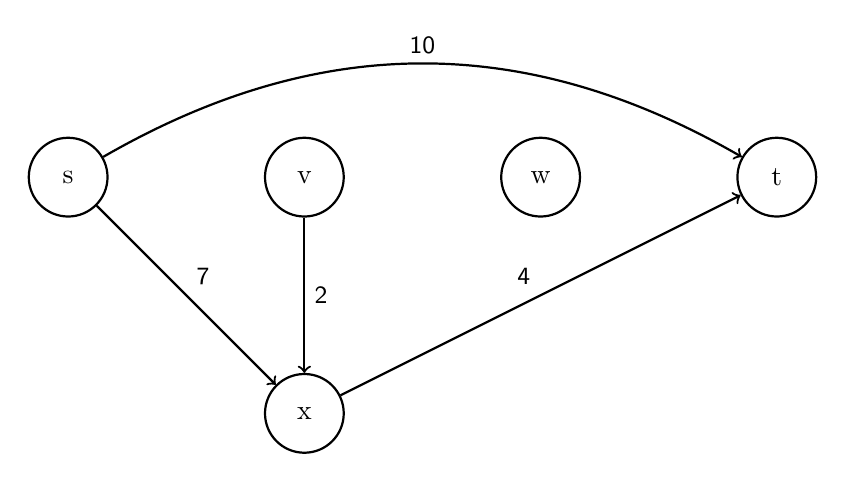
\begin{tikzpicture}[->, auto, node distance=3cm, thick, main node/.style={circle, draw, minimum size=1cm}]
        \node[main node] (s) {s};
        \node[main node] (v) [right of=s] {v};
        \node[main node] (w) [right of=v] {w};
        \node[main node] (t) [right of=w] {t};
        \node[main node] (x) [below of=v] {x};
    

        \path[every node/.style={font=\sffamily\small}]
        (s) edge node {7} (x)
        (v) edge node {2} (x)
        (x) edge node {4} (t)
        (s) edge [bend left] node {10} (t);

    \end{tikzpicture}
    \caption{Nuevo grafo sin aristas st-eficientes}
    \label{fig:new}
\end{figure}

En el primer gráfico (\ref{fig:original}), las aristas rojas representan el camino mínimo original que es st-eficiente. En el segundo gráfico (\ref{fig:new}), se muestran las aristas del nuevo grafo que no son st-eficientes, y sobre el cual se debe ejecutar el algoritmo de Dijkstra para encontrar el camino mínimo.

\end{document}
